%!TEX root = ../../Main.tex
\graphicspath{{Chapters/Systemforlob/}}
%-------------------------------------------------------------------------------

\section{Systemidentification}

\subsection{Kontinuer controller design}

For at kunne estimere dette system, er det første som skulle laves en overføringsfunktion, for den motor som blev brugt til projeketet. Her stødte gruppen på det første problem med systemet, da det ikke var stabilt. Gruppen blev derfor nød til at indsætte fjedre, for at sikre at systemet var stabilt i en stationær position. Hertil blev der valgt at tilføje en elastik til hver side af bilen, for at opfylde ønsket om et stabilt stationær system. 
Herefter blev målingen lavet for at identificere, en overføringsfunktion for motoren. Da dette system, både skal kunne gå mod højre og venstre, blev der påført et firkantsignal. Herunder ses, hvordan dynamikken i motorens tagometer blev genereret gennem firkantsignalet.      
   

\begin{figure}[H]
	\centering
	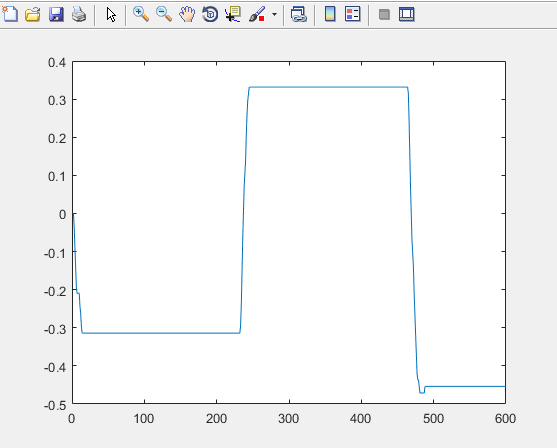
\includegraphics[width = 300pt]{Img/system_respons}
	\caption{System Respons}
	\label{fig:system_respons}
\end{figure}

Overføringsfunktionen bliver genereret ud fra funktionen tfest(), som estimerer en overføring. Hertil får vi overføringsfunktionen:

\begin{equation}
  Tf(s) = \frac{5.029}{s^2 + 39.28 s + 717.9}
\end{equation}

I forhold til vores krav, forsøges der at placere poler til systemet. Dette laves ud fra udregningen: 


\begin{equation}
  G(s) = \frac{wn^2}{s^2+2*\zeta*wn*s+wn^2}
\end{equation}

Hvor wn beregnes ud fra ligningen:

\begin{equation}
  wn = \frac{4}{\zeta*Ts}
\end{equation} 

Og zeta, også kaldet damping ratio beregnes ud fra: 
\begin{equation}
  \zeta = \frac{-\ln(OS/100)}{sqrt{\pi^2+\ln^2(OS/100)}}
\end{equation} 

ud fra de kravene - Settling Time (Ts) og damping ratio, beregner vi derved poler som ligger i -4\textpm\ 4.08i. 

\subsection{state space}

I dette projekt bliver systemet controller del repræsenteret på controller state space form, dette gøres for at kunne ændre på state vectorerne, som ændres vha. gainblokke (K), som bliver tilføjet til systemet. For at transformere transferfunktionen til en state space model, laves en state space tranformation i matlab. State space formlen giver statestene: 

\begin{enumerate}
 
\item
 $
A = 
\begin{bmatrix}

	-39.2765 & -717.8563 \\
    1.0000     &    0
\end{bmatrix}
     $
\item
 $
B = 
\begin{bmatrix}

	1\\
    0
\end{bmatrix}
     $    
  
\item 
 $
C = 
\begin{bmatrix}

	0  &  5.0293
\end{bmatrix}
     $    
 \item
 $
D = 
\begin{bmatrix}

	0  
\end{bmatrix}
     $  
\end{enumerate}      
Som vist tidligere, er der beregnet nogle poler, som ønskes. Derfor indsættes en K matrix, som skal placeres, i tilbagekoblingen for at opnå de øsnkede poler i close loopet, dette ses nedenunder. 

\begin{lstlisting}
K = place(A,B,poles);
AA = A-B*(K);
sys=ss(AA,B,C,D);
\end{lstlisting}

Herved vises closed loop repræsentationen, for controller design, ift. kravene på overshoot og settling time.\\


HEREFTER KAN VI TILFØJE EN Ke, som regulerer på STEADY STATE ERROR (MANGLER KODE HERFRA). 

\subsection{Diskret controller design}
For at kunne implementere systemet på en microcontroller - som på LEGO V3, kan der med fordel transformeres til diskrete states. Dette kommer af at reguleringen skal foregå på et digitalt system, som sampler med en bestemt frekvens. 
Både overføringsfunktionen og state space repræsentationen bliver transformeret til diskrete værdier, samt gøres vores poler, hvormed K værdierne ændres til de passende værdier. Alt dette gøres igennem matlab, hvor funktionen c2d bliver brugt. 

\subsection{Observer design}
Da systemet i praksis foregår på en motorblok, kan vi ikke hente de states matrixen, da x1 og x2 er en del  af systemet, ift ligningen for state space controller repræsentationen: 
\begin{gather}
  \dot{x}=Ax+Bu \\
  y=Cx
\end{gather}
Derfor indsættes yderligere en blok i systemet, for at kunne observere ind og output, og på baggrund af dem, og de beregnede state matrixes, beregnes en estimeret xhat, som skal bruges til tilbagekoblingen. \\
Observer formlen hedder:


\begin{gather}
  \dot{\hat{x}}=A\hat{x}+Bu+L(y-\hat{y}) \\
  \hat{y}=C\hat{x}
\end{gather}

Vha af mellemregninger, får vi formlen: 
\begin{gather}
  \dot{\hat{x}}=(A+BK-LC)\hat{x}+Ly \\
  u=K\hat{x}
\end{gather}
Som er den formlen vi bruger til at lave vores observer.

 